\documentclass[12pt,fleqn]{article}\usepackage{../common}
\begin{document}
Ders 12

Zincirleme Kanunu hatirlayalim

\[ \frac{dw}{dt}  = w_x \frac{dx}{dt} + 
w_y \frac{dy}{dt} + 
w_z \frac{dz}{dt}  \]

Bu formul, kismi turevler uzerinden, $w$'daki degisimin $x,y,z$'deki
degisime ne kadar ``hassas'' ne kadar ``bagli'' oldugnu gosteriyor.

Simdi usttekini daha azaltilmis, ozetli (compact, concise) bir formda soyle
yazacagim. 

\[ = \nabla w \cdot  \frac{d\vec{r}}{dt} \]

Gradyan vektoru tum kismi turevlerin bir araya konmus halidir. 

\[ \nabla w = <w_x, w_y, w_z> \]

Tabii ki bunu soyleyince ustteki gradyan'in $x,y,z$'ye bagli oldugunu da
soyluyoruz, mesela $w$'nun belli bir nokta $x,y,z$'da gradyanini
alabilirsiniz, o zaman her degisik $x,y,z$ noktasinda farkli bir vektor
elde edersiniz, ki bu vektorlerin tamamina ileride ``vektor alani (vector
field)'' ismini verecegiz. Devam edelim, 

\[ \frac{d\vec{r}}{dt} = < \frac{dx}{dt}, \frac{dy}{dt}, \frac{dz}{dt} > \]

Yani hiz vektoru (velocity vector) $d\vec{r}/{dt}$ yukaridaki gibi
tanimlidir.

Bugunku amacimiz gradyan vektorunu anlamak, ve nerelerde
kullanabilecegimizi incelemek. Gradyanlari yaklasiksal formullerde
kullanmak mumkundur, vs. Ustte gordugumuz onun notasyonu. 

Gradyanlarin belki de en ``havali'' ozellikleri sudur. 

Teori

Iddia ediyorum ki $\nabla w$ vektoru, $w = \textrm{ bir sabit }$ile elde
edilecek kesit yuzeyine (level surface) her zaman diktir.

Eger fonksiyonumun bir kontur grafigini cizersem

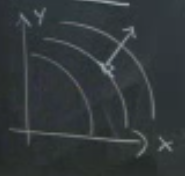
\includegraphics[height=3cm]{12_1.png}

gosterilen noktada hesaplanacak gradyan vektoru o noktadaki kontura
diktir. 

Ornek 1

Lineer bir $w$ kullanalim. 

\[ w = a_1 x + a_2 y + a_3 z \]

Gradyan nedir? Kismi turevleri alalim:

\[ \nabla w = <a_1, a_2, a_3> \]

Konturlari nasil elde ederim? $a_1 x + a_2 y + a_3 z  = c$ ki $c$ bir
sabittir, bu formulu tatmin eden tum $x,y,z$ degerleri bir duzlem
olustururlar. 

Bu duzlemin normalinin nasil alinacagini biliyoruz, katsayilara bakariz,
$<a_1,a_2,a_3>$. Bu vektorun gradyanla ayni ciktigina dikkat, ki normal
vektor de duzleme diktir zaten. Ayni cikmalari mantikli. 

Aslinda bu ornek gradyanin dikligini bir anlamda ispatliyor, cunku duzlem
olmasa bile herhangi bir fonksiyonun birinci yaklasiksalligi bir duzlem
yaratir, o duzlemin normali, gradyani esitligi bizi yine gradyanin
dikligine goturur. Ama bu yeterince ikna edici olmadiysa baska bir ornege
bakabiliriz. 

Ornek 2

\[ w = x^2 + y^2 \]

Bu fonksiyonun kesit seviyeleri, degisik yaricaplara sahip dairelerdir,
$x^2 + y^2 = c$ formulundeki degisik $c$ degerleri bu daireleri tanimlar. 

Gradyan vektoru

\[ \nabla w = <2x, 2y> \]

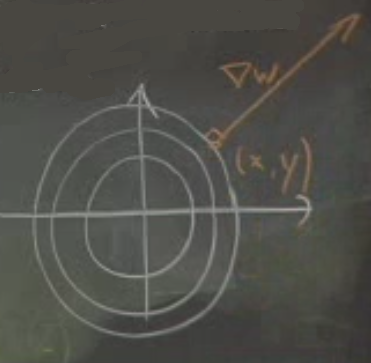
\includegraphics[height=4cm]{12_2.png}

Secilen $x,y$ noktasinda $\nabla w$ gosterilmis. Bu vektorun $x$ ve $y$
eksenlerinde boyunun, basladigi noktaya gore olan $x,y$ degerlerinin
yaklasik iki kati olduguna dikkat, ki bu da $<2x,2y>$ vektoru ile uyumlu. 

Simdi gradyanin niye kesit egrilerine hep dik oldugunu ispatlayalim.

Ispat

Once kesit egrileri ``uzerinde'' hareket eden bir nokta hayal edecegiz. Bu
nokta fonksiyonun sabit oldugu yerlerden geciyor demektir, cunku kontur
uzerinde fonksiyon degeri hep aynidir. 

Egri $\vec{r} = \vec{r}(t)$ hep $w = c$ uzerinde olacak. Resme bakalim,
hayali bir kesit yuzeyi uzerinde bir egri bu (kirmizi renkli) ve bu egrinin
uzerinde giden noktanin bir hizi olacak. Bu arada $w$ mesela $w = x^2 +
y^2$ belki,
herhangi bir uc boyutlu fonksiyon. $\vec{r}$'nin $w$ ustunde gitmesi demek, $\vec{r}$ ile 
$w$ parametrize edilebilir demek, $\vec{r}(t)
= <x(t),y(t),z(t)>$ ve onu 
kullanarak $w(\vec{r}(t)) = c$.

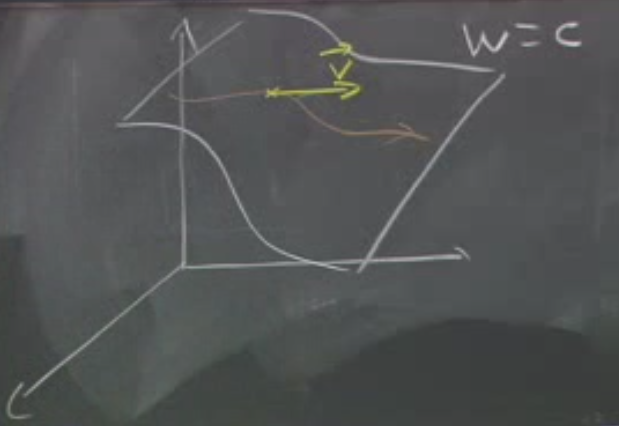
\includegraphics[height=4cm]{12_3.png}

Iddia o ki, 

\[ \vec{v} = \frac{d\vec{r}}{dt} \]

vektoru, kesit $w = c$'ye muhakkak teget olmali, cunku hiz egriye teget, ve
egri kesit icinde. Bu arada $w$'nin aslinda $w(\vec{r}(t))$ oldugunu
belirttik.

Bu sayede Zincirleme Kanununu kullanarak 

\[ \frac{dw(\vec{r})}{dt} = \nabla w \cdot \frac{d\vec{r}}{dt} = \frac{dc}{dt}\]

esitligini kurabiliriz. Noktasal carpim nereden geldi? Bu ifade $w$'nin
her kismi turevinin alip, ona tekabul eden $\vec{r}(t)$ ogesinin turevi ile
carpip sonuclarin toplanmasi demek. Sonuc Zincirleme Kanunu'ndaki goruntu
olacaktir. Ayrica

\[  = \nabla w \cdot \vec{v} = 0\]

Sifira esitligin sebebi $w = c$ olmasi ve sabitin turevi $dc/dt$ sifir oldu. 

Simdi sifir sonucundan ters yone gidelim: iki vektorun noktasal carpimi ne
zaman sifir sonucu verir? Eger vektorler birbirine dik ise. Demek ki
$\nabla w \perp \vec{v}$.

Hatta iddia ediyorum ki bu diklik $w=c$ uzerindeki her hareket (motion)
icin gecerlidir. Yani $\vec{v}$, kesit yuzeyine teget olan herhangi bir
vektor olabilir, ustteki diklik hep dogru olacaktir.

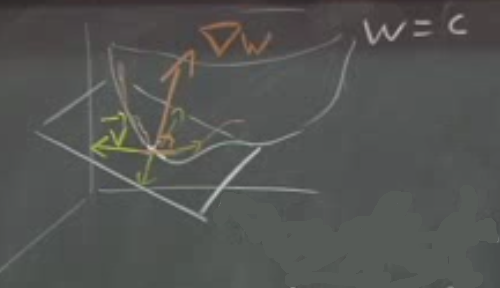
\includegraphics[height=4cm]{12_4.png}

Bunun guzel bir uygulamasi su, artik istedigimiz her seyin teget duzlemini
bulabiliriz. 

Ornek

Yuzey $x^2 + y^2 - z^2 = 4$'un $(2,1,1)$ noktasindaki teget duzlemini
bul. Alttaki sekil bir hiperboloid (hyperboloid) ve bu dersin altinda
grafiklemek icin gereken kodlar var. 

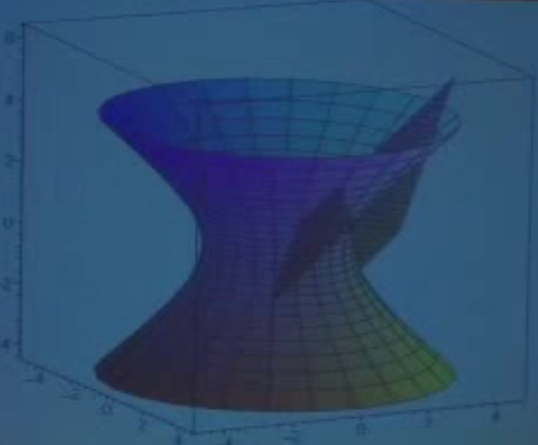
\includegraphics[height=4cm]{12_5.png}

Resimde teget duzlem pek teget gibi degil, diger grafigin icine girmis gibi
duruyor, fakat problemin verdigi noktada duzlem teget. 

Bu duzlemi nasil bulacagiz? Gradyani hesaplayarak. 

Kesit seviyesi $w=4$ ve Yuzey $w = x^2 + y^2 - z^2$. 

\[ \nabla w = <2x, 2y, -2z> \]

Verilen nokta degerlerini bu gradyan vektorune verirsek, sonuc
$<4,2,-2>$. Bu sonuc yuzeye ya da teget duzleme normal (dik) olan 
vektoru verecek. 

Bu normal vektoru kullanarak duzlemin formulunu bulabiliriz. 

\[ 4x + 2y - 2z = ? \]

Soru isareti ne olur? $(2,1,1)$ noktasini formule koyarsak, sonuc 8 cikar.

\[ 4x + 2y - 2z = 8 \]

Alternatif Yontem

Aslinda tum bunlari gradyan olmadan da yapabilirdik, bir diferansiyel ile
ise baslayabilirdik

\[ dw = 2x dx + 2y dy -2z dz \]

$(2,1,1)$ noktasinda

\[ = 4dx + 4dy - 2dz \]

Yaklasiksal olarak 

\[ \Delta w \approx 4 \Delta x + 2\Delta y - 2\Delta z  \]

Ne zaman kesit yuzeyi, kontur uzerindeyiz? Eger $w$'de hic degisim yok ise,
yani $\Delta w = 0$ ise. Bu arada ustteki yaklasiksalligin bir lineer
yaklasiksallik oldugunu unutmayalim. $(2,1,1)$ noktasinda bu tegeti
kullanmak istersek,  $\Delta w = 0$ esitligi bize $4 \Delta x + 2\Delta y -
2\Delta z $ 
teget duzlemini verecektir. Nasil? $\Delta x$ degisimdir, teget duzlem
uzerinde degisimi tanimlamak istiyorsak, $(2,1,1)$'den baslayarak bir yere
gittigimizi dusunmemiz gerekir, ki mesela $x-2$ degisimini yapabiliriz,
vs. Tam formul

\[ 4(x-2) + 2(y-1) - 2(z-1) = 0 \]

Yonsel Turevler (Directional Derivatives) 

Elimdeki bir $w = w(x,y)$ formulunun kismi turevini aldigim zaman 
$\partial  w/\partial x$, $\partial w/\partial y$ ile mesela, bu turevler x-ekseni ya da y-ekseni 
yonunde degisim oldugu zaman $w$'nun nasil degistini olcerler. Peki baska
yonlere gore, mesela bir birim vektor $\hat{u}$ yonunde turev alinamaz mi? 
Cevap evet. Yonsel turevler bu ise yariyorlar. 

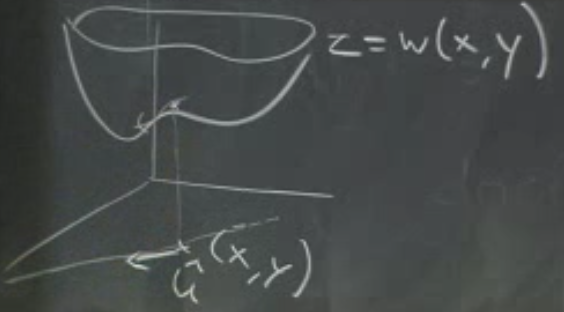
\includegraphics[height=4cm]{12_6.png}

Yani $\hat{u}$ uzerinden gecen yolda ilerlerken $z$'nin nasil degisecegini
merak ediyorum. Duz cizgi uzerindeki gidisata (straight line trajectory)
bakiyoruz.

$s$ adli bir parametreye bagli bir pozisyon vektoru $\vec{r(s)}$ hayal
edelim, oyle ki,

\[ d\vec{r}/ds = \hat{u} \]

sonucunu versin.

Niye ustte $t$ yerine $s$ kullandim? Cunku cizgi boyunca birim hizda
ilerliyorum, o zaman parametrize ettigim sey katedilen yol. $s$ bir anlamda
egri uzunlugu (arc length), tabii tam egri denemez cunku cizgi duz, ama
yine mesafe kavramini kullaniyoruz.

O zaman $dw/ds$ nedir? Bunu hesaplamak icin Zincirleme Kanunu'nun ozel bir
durumunu kullanacagiz.

Eger $\hat{u} = <a,b>$ ise

\[ x(s) = x_0 + as \]

\[ y(s) = y_0 + bs \]

Bu formulleri $w$'ye sokariz, sonra $dw/ds$'i hesaplariz. 

Tanim: Yonsel Turev

\[ \frac{dw}{ds}_{|\hat{u}} \]

Daha once kismi turevleri incelerken onlari geometrik olarak, x ve y
eksenine paralel duzlemlerin fonksiyonu kesmesi olarak gormustuk. Yonsel
turevler ise herhangi bir yondeki (daha dogrusu $\hat{u}$ yonundeki) bir
duzlemin fonksiyonu kesmesi olarak gorulebilir.

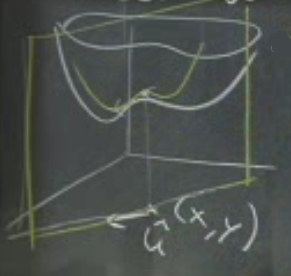
\includegraphics[height=4cm]{12_7.png}

Tanim

$dw / ds_{|\hat{u}}$ = Bir grafigin (fonksiyonun) $\hat{u}$ vektorunu
iceren / ona paralel olan, ve dikey duzlem (vertical plane) kesilmesi ile
elde edilen, o duzlemdek yansimasinin olusturdugu egrinin degisimi / egimi
(slope).

Zincirleme Kanunu uygulanirsa

\[ \frac{dw}{ds} = \nabla w \cdot \frac{d\vec{r}}{ds} 
= \nabla w \cdot \hat{u}
\]

Hatirlamamiz gereken formul o zaman

\[ \frac{dw}{ds}_{|\hat{u}} =  \nabla w \cdot \hat{u} \]

Esitligin sag tarafi ``gradyanin $\hat{u}$ yonunde giden bileseni, kismi''
olarak ta nitelenebilir. 

Kavramlarin birbiriyle alakasini iyice gormek icin suna bakalim

Ornek

\[ 
\frac{dw}{ds}_{|\hat{i}} =  \nabla w \cdot \hat{i} = 
\frac{\partial w}{\partial x} \]

Geometrik olarak

\[ \frac{dw}{ds}_{|\hat{u}} =  \nabla w \cdot \hat{u} \]

\[ =  |\nabla w||\hat{u}|\cos(\theta)  \]

$\hat{u}$ birim vektor olduguna gore $|\hat{u}| = 1$, formulden atilir

\[ =  |\nabla w||\cos(\theta)  \]

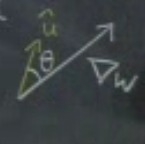
\includegraphics[height=2cm]{12_8.png}

Bu ifade ``gradyanin $\hat{u}$ yonundeki bileseni'' hesabinin bir diger
versiyonudur aslinda. 

Su soruyu soralim: hangi yondeki degisim en buyuktur? $|\nabla
w||\cos(\theta)$ ifadesinin
en buyuk oldugu yer $\cos(\theta)=1$ oldugu zamandir, yani $\theta = 0$, ki
bu durum $\hat{u} = dir(\nabla w)$, yani $\hat{u}$'nun gradyan ile ayni
yonde oldugu zamandir. 

O zaman su yorumu da yapabiliriz, gradyan belli bir noktada fonksiyonun en
cok artacagi yonu gosterir. 

Peki $|\nabla w|$, yani $\nabla w$'nun buyuklugu neye esittir? 

\[ |\nabla w| =   \frac{dw}{ds}_{|\hat{u}=dir(\nabla w)}  \]

En hizli dusus (azalis) hangi yondedir? En fazla artisin tam tersi
yonunde. 

Yani min $dw/ds_{|\hat{u}}$ icin $cos(\theta) = -1$ olmalidir, yani $\theta =
180^o$,  $\hat{u}$, $-\nabla w$ 
yonunde oldugu zaman.

Peki su ne zaman dogrudur? 

\[ \frac{dw}{ds}_{|\hat{u}} = 0 \]

Yani fonksiyon hangi yonde degismez? 

Bunun icin $\cos(\theta) = 0$ olmalidir, ki bu $\theta = 90^0$ oldugu
zamandir. Yani $\hat{u} \perp \nabla w$ ise. Bunu anlamanin bir diger yolu,
hic degisimin olmadigi yonun kesit yuzeyine teget oldugudur, bu yuzeyde $w$
hic degismedigine gore degisim olmaz, degisim yoksa, biz de teget hareket
ediyoruz demektir. 

Soru

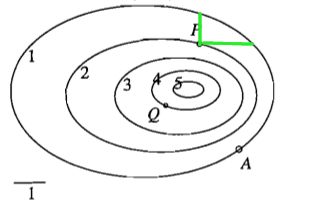
\includegraphics[height=3cm]{2d9.png}

P noktasinda $\partial w/ \partial x$ ve $\partial w/\partial y$'yi kabaca hesapla. 

\[ \frac{\partial w}{\partial x} = \frac{dw}{ds} \bigg|_{\hat{i}} \approx
\frac{\Delta w}{\Delta s} \approx
\frac{-1}{5/3} = -0.6
\]

\[ \frac{\partial w}{\partial y} = \frac{dw}{ds} \bigg|_{\hat{j}} \approx
\frac{\Delta w}{\Delta s} \approx
\frac{-1}{1} = -1
\]

$\Delta = -1$ cunku dik giderken kesit seviye 2'den 1'e geliyoruz, $w$ 1
azaliyor. Bu gidisat $s$'in kendi degisimi $\Delta s$, bunu da kabaca, sol
alt kosedeki skalaya bakarak tahmin ediyoruz, saga dogru yatay gidis 1'den
buyuk gibi duruyor, ona 5/3 demisiz, yukari dogru gidisat tam 1 gibi
duruyor, ona 1 demisiz. 

$\partial w / \partial y$ hesabinda niye asagi degil yukari gitmisiz? Cunku
$\hat{i}$'nin yonu yukaridir, asagi degil. 


Hiperboloid 

Parametrizasyonu turetelim. Diyelim ki $x^2 + y^2 - z^2 = 1$ gibi bir
paraboloid'imiz var. $x,y$'yi soyle alalim

\[ x = r \cos u \]

\[ y = r \sin u \]

Yerine koyarsak

\[ r^2 - z^2 = 1 \]

elde ederiz. Simdi kareleri birbirinden cikartilinca 1 veren bir seyler
bulmak lazim. Hiperbol sin ve cos (hyperbolic sine, cosine) boyle
fonksiyonlardir. 

\[ \cosh^2x - \sinh^2x = 1 \]

Bu esitligi kullanarak 

\[ r = \cosh v \]

\[ z = sinh(v) \]

Yine yerine koyalim

\[ x = \cos u \cosh v \]

\[ y = \sin u \cosh v \]

\[ z = \sinh v \]

Son formullerimiz bunlar.

\begin{minted}{python}
from __future__ import division

from mpl_toolkits.mplot3d import Axes3D

fig = plt.figure(figsize=plt.figaspect(1))  # Square figure
ax = fig.add_subplot(111, projection='3d')

r=1;
u=np.linspace(-2,2,200);
v=np.linspace(0,2*np.pi,60);
[u,v]=np.meshgrid(u,v);

a = 1
b = 1
c = 1

x = a*np.cosh(u)*np.cos(v)
y = b*np.cosh(u)*np.sin(v)
z = c*np.sinh(u)

ax.plot_surface(x, y, z,  rstride=4, cstride=4, color='b')

plt.savefig('hyperboloid.png')
\end{minted}

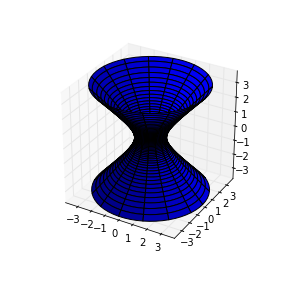
\includegraphics[height=6cm]{hyperboloid.png}

Bir diger kod $a \cos,b \sin$ ifadelerinin toplamini gosteriyor

\begin{minted}{python}
from pylab import *

xmax = 6.
xmin = -6.
D = 100
x = linspace(xmin, xmax, D)

a = 3
b = 1

plot(x, (a*cos(x) + b*sin(x)))
plot(x, (a*cos(x)))
plot(x, (b*sin(x)))

grid()
legend(['sum', 'cos','sin'])
plt.savefig('1h7.png')
\end{minted}

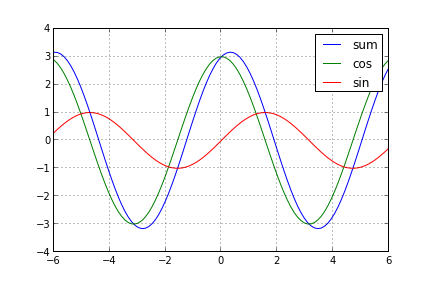
\includegraphics[height=6cm]{1h7.png}

\end{document}
